% Chapter 6

\chapter{Spracovanie dát a zobrazenie získanych parametrov štruktúr MOS.} % Main chapter title

\label{Chapter6} % For referencing the chapter elsewhere, use \ref{Chapter1} 

\lhead{Chapter 6. \emph{Spracovanie dát a zobrazenie získaných parametrov štruktúr MOS}}

V tejto kapitole uvedieme stručne postup spracovania dát, nameraných
pomocou programov zberu dát a zameriame sa na plošné zobrazenie
získaných parametrov štruktúr MOS. Metodika výpočtu parametrov
štruktúr MOS bola popísaná v kapitolách 3 a 4, na ktoré sa budeme
odvolávať.

Väčšina parametrov je určovaná z nameraných dát pomocou samostatných
programov a ukladaná do dátových súborov, ktorých štruktúra bola
popísaná v časti 5. Plošné rozloženie vypočítaných parametrov štruktúr
MOS možno potom zobraziť na displeji počítača. Pri zobrazovaní na
displeji je k dispozícii 16 farieb, avšak pri zobrazení obrázkov na
tlačiarni bolo kvôli lepšej rozlišiteľnosti použitých len 6
farieb. Orientácia kremíkovej dosky na obrázkoch je smerom 'fazetou
hore', pričom jeden štvorček zobrazenej plochy predstavuje hodnotu
parametra štruktúry MOS. Farba štvorčeka závisí od intervalu, do
ktorého daná hodnota spadá. Škála intervalov je zobrazená v pravej
časti obrázku, pričom číslo uvedené pri jednotlivých farbách
predstavuje dolnú hranicu intervalu. Pretože sa farby v škále
intervalov viackrát opakujú, bolo potrebné označiť, v ktorých
intervaloch sa zobrazované hodnoty nachádzajú. To je označené veľkým
písmenom 'X' medzi dolnou hranicou intervalu a prislúchajúcou
farbou. Možno ešte poznamenať, že náhodne odlišné výsledky v
niektorých bodoch kremíkovej dosky spôsobia, že sa v škále intervalov
objaví vyznačený interval, ktorý zjavne nesúvisí s ostatnými
hodnotami, čo možno pripísat nefunkčnej štruktúre MOS. Treba ešte
upozorniť, že orientácia škály sa môže pri zobrazení rôznych
parametrov meniť.

\section{Určenie koncentračného profilu dotujúcich prímesí, dávky implantácie a napätia vyrovnaných pásov.}\label{sec:6.1}

Určenie koncentračného profilu dotujúcich prímesí vykonáva samostatný
program, ktorý ako vstupné dáta vyžaduje súbory (a) nameraných HF C-V
závislostí a (b) nameraných kapacít oxidovej vrstvy štruktúry
MOS. Výstupom programu je dátový súbor obsahujúci hĺbkové priebehy
koncentračných profilov skúmaných štruktúr MOS, ktoré sú počítané
podľa vzťahov uvedených v časti \ref{sec:4.1}. Ak boli v procese zberu
dát zmerané aj kvázistatické C-V závislosti, program vykoná korekciu
koncentračného profilu na hustotu pascí rozhrania
$Si-SiO_2$. Povrchový potenciál určujeme podľa vzťahov \ref{eq:4.3} a
\ref{eq:4.4} a používame ho pre korekciu aproximácie hlbokého
ochudobnenia pri povrchu polovodiča a pre výpočet hĺbky (šírky
OPN). Vedľajším produktom je dátovy súbor obsahujúci napätia
vyrovnaných pásov $V_{fb}$, ktoré sa určujú v bode C-V závislosti, pre
ktoré povrchový potenciál $\varphi_s$ mení znamienko. Obrázok
\ref{fig:6.1} predstavuje plošné rozloženie koncentrácie v rôznych
hĺbkach polovodiča a na obrázku \ref{fig:6.2} je znázornené rozloženie
$V_{fb}$. Koncentračný profil prímesí bol vytvorený implantáciou
$P^{31}$ s dávkou $4.0\times 10^{15} m^{-2}$ pri energii $120
keV$. Aktivácia prebiehala počas 40 minút pri teplote $1050 \degree C$
v atmosfére $N_2$. Stredná hodnota $N(x)$ je spolu s ďalšími priebehmi
pre rôzne implantačné dávky zobrazená na obrázku \ref{fig:7.3}.

Pre známe priebehy koncentračných profilov môžeme vypočítať dávku
implantácie podľa vzťahu

\begin{equation}\label{eq:6.1}
D = \int_{0}^{x_{1}}(N(x) - N_{b}) dx
\end{equation}

kde predpokládame, že poznáme priebeh N(x) do vzdialenosti $x_{1}$ ,
pre ktorú platí

\begin{equation}\label{eq:6.2}
N(x) = N_{b} \qquad {x \ge x_{1}}
\end{equation}

Dávka $D$ vypočítaná týmto spôsobom predstavuje časť implantovaných
iónov, ktoré sa dostali v priebehu implantácie do polovodiča a boli
aktivované v poimplantačnom tepelnom spracovaní. Na obrázku
\ref{fig:6.3} je znázornené plošné rozloženie dávky na testovanej
kremíkovej doske určenej zo závislosti $N(x)$ zobrazených na obrázku
\ref{fig:6.1}.

\begin{figure}[h!]\centering
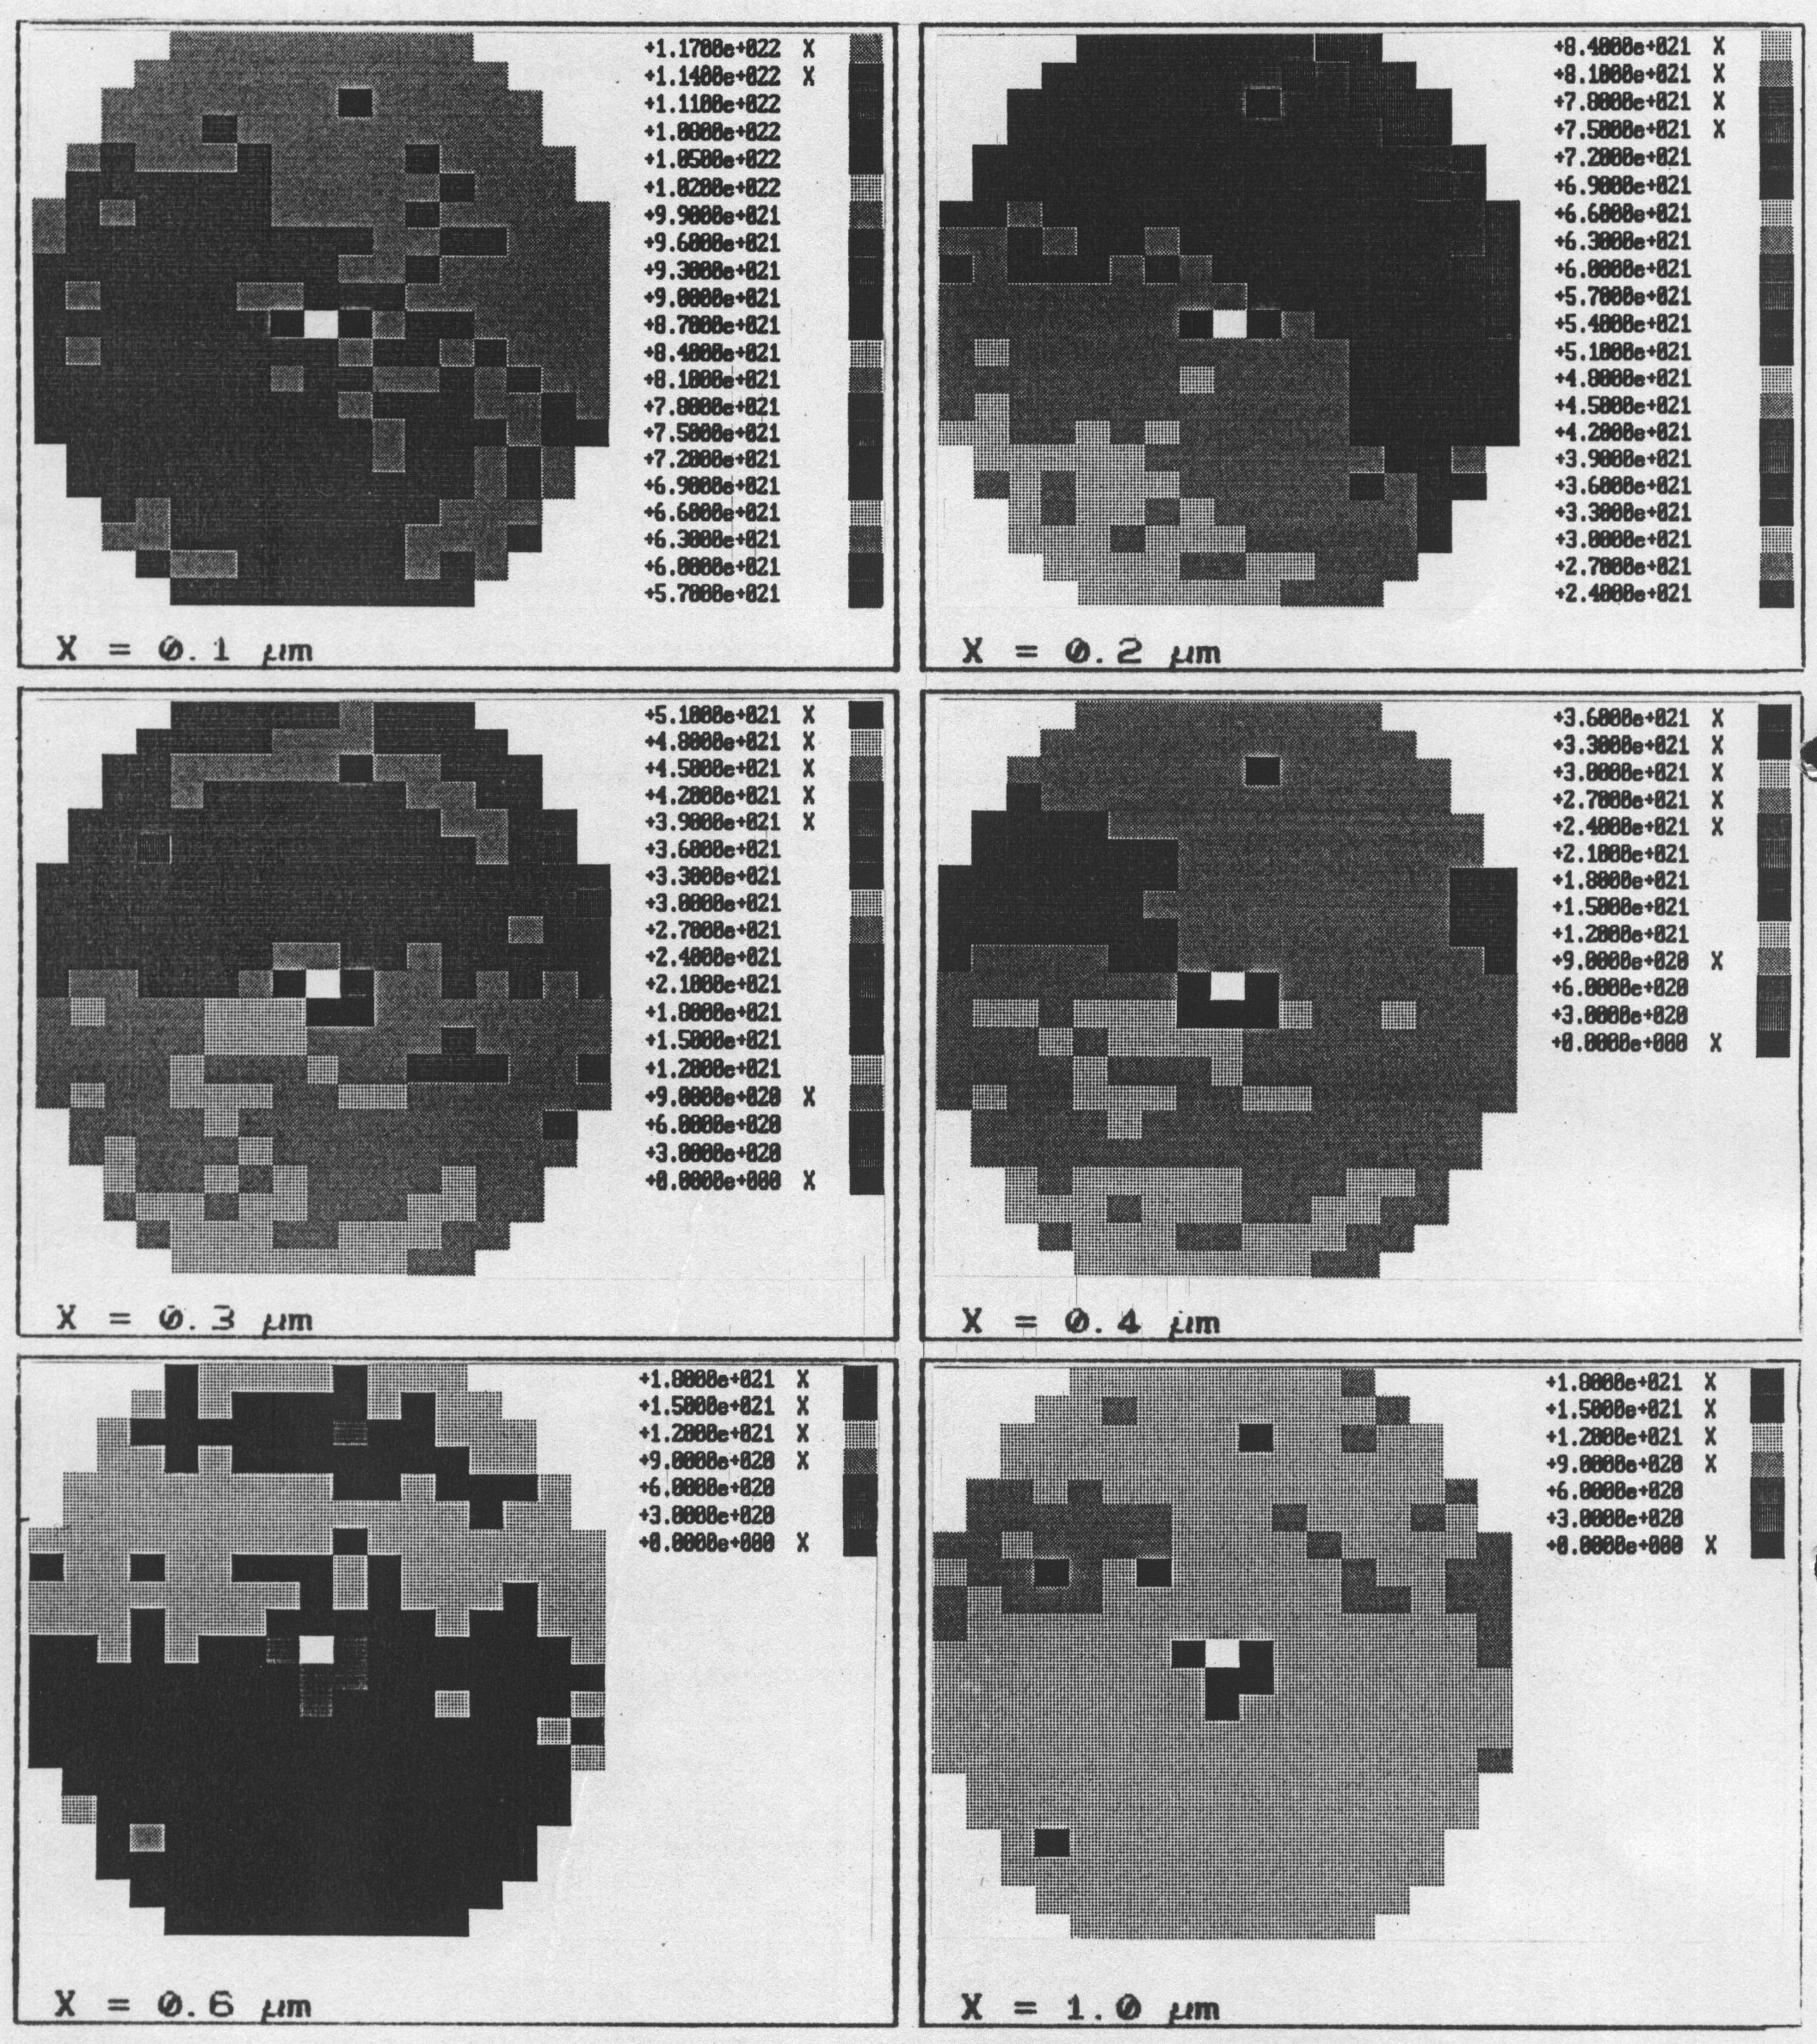
\includegraphics{Figures/fig-6-1.eps}
\captionsetup{justification=raggedright, singlelinecheck=false}
\caption[Rozloženie dotujúcich prímesí $N(x)$ v rôznej hĺbke
  $x$]{Rozloženie dotujúcich prímesí $N(x)$ v rôznej hĺbke $x$ pod
  povrchom polovodiča pre dávku implantácie $4.0 \times 10^{15}
  m^{-2}$.}
\label{fig:6.1}
\end{figure}

\begin{figure}[h!]\centering
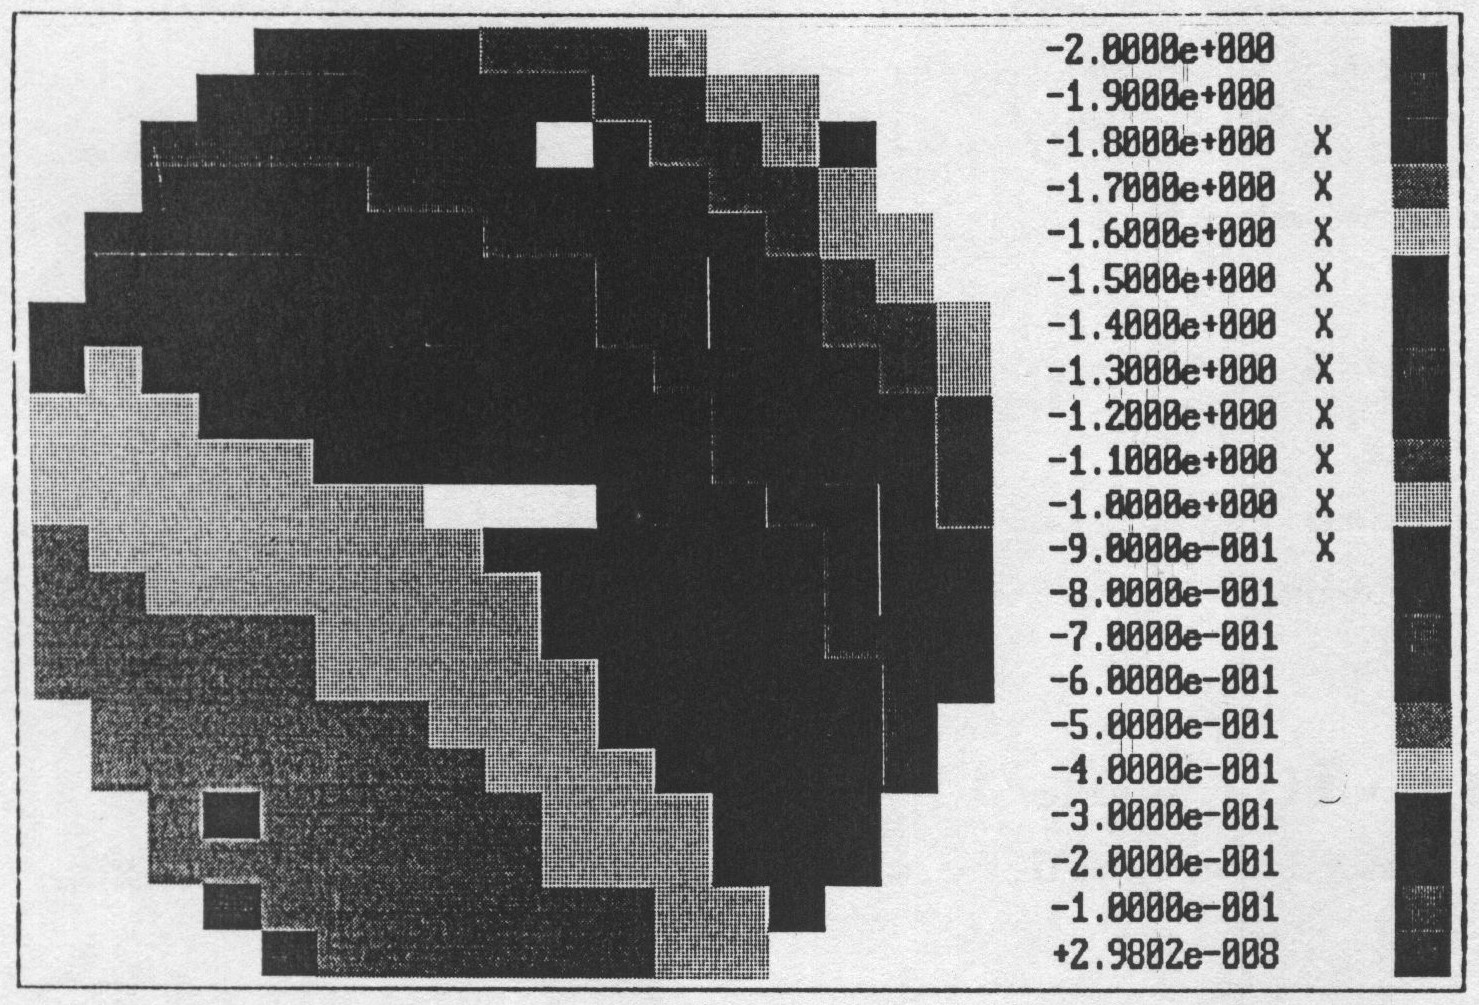
\includegraphics{Figures/fig-6-2.eps}
\captionsetup{justification=raggedright, singlelinecheck=false}
\caption[Plošné rozloženie $V_{fb}$]{Plošné rozloženie $V_{fb}$ určené
  pri výpočte $N(x)$ z obrázka \ref{fig:6.1}.}
\label{fig:6.2}
\end{figure}

\begin{figure}[h!]\centering
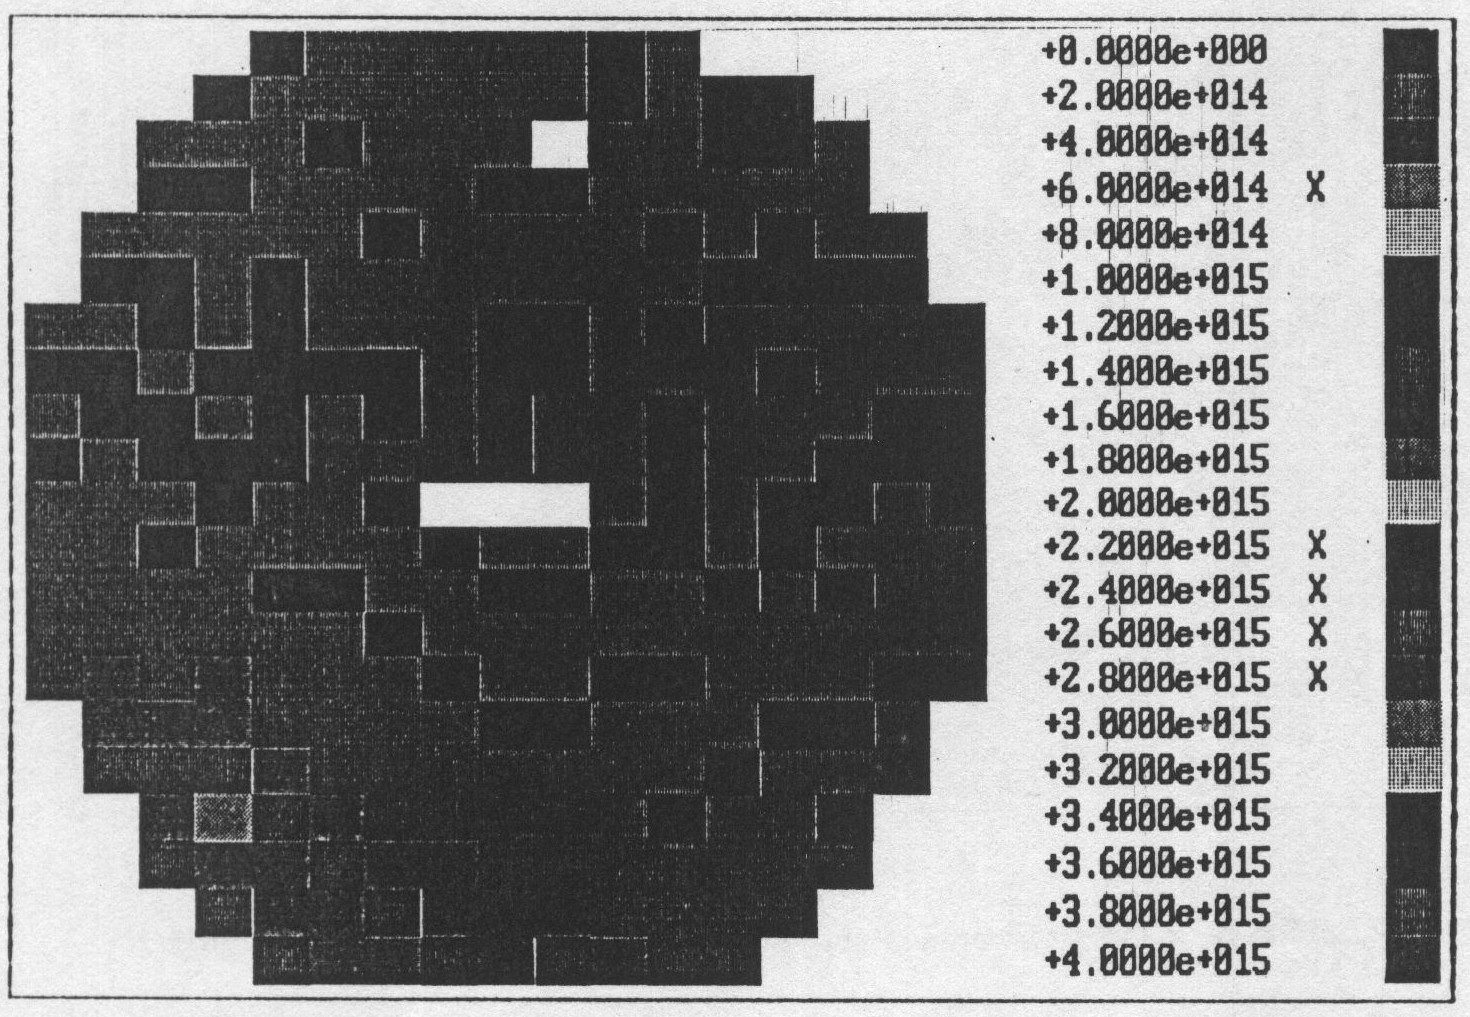
\includegraphics{Figures/fig-6-3.eps}
\captionsetup{justification=raggedright, singlelinecheck=false}
\caption[Plošné rozloženie nameranej dávky implantácie]{Plošné
  rozloženie nameranej dávky implantácie pre profil N(x) z obrázka
  \ref{fig:6.1}.}
\label{fig:6.3}
\end{figure}


\section{Určenie hrúbky oxidovej vrstvy.}\label{sec:6.2}

Ak poznáme kapacitu oxidovej vrstvy štruktúry MOS a jej plochu, potom
môžeme vypočítať jej hrúbku podľa vzťahu

\begin{equation}\label{eq:6.3}
h_{ox} = A \frac{\epsilon}{C_{ox}}
\end{equation}

kde sme použili hodnotu relatívnej permitivity $SiO_{2}$
$\epsilon_{r}=3.9$. Plošné rozloženie hrúbky oxidovej vrstvy je potom
zobrazené na obrázku \ref{fig:6.4}.

\begin{figure}[h!]\centering
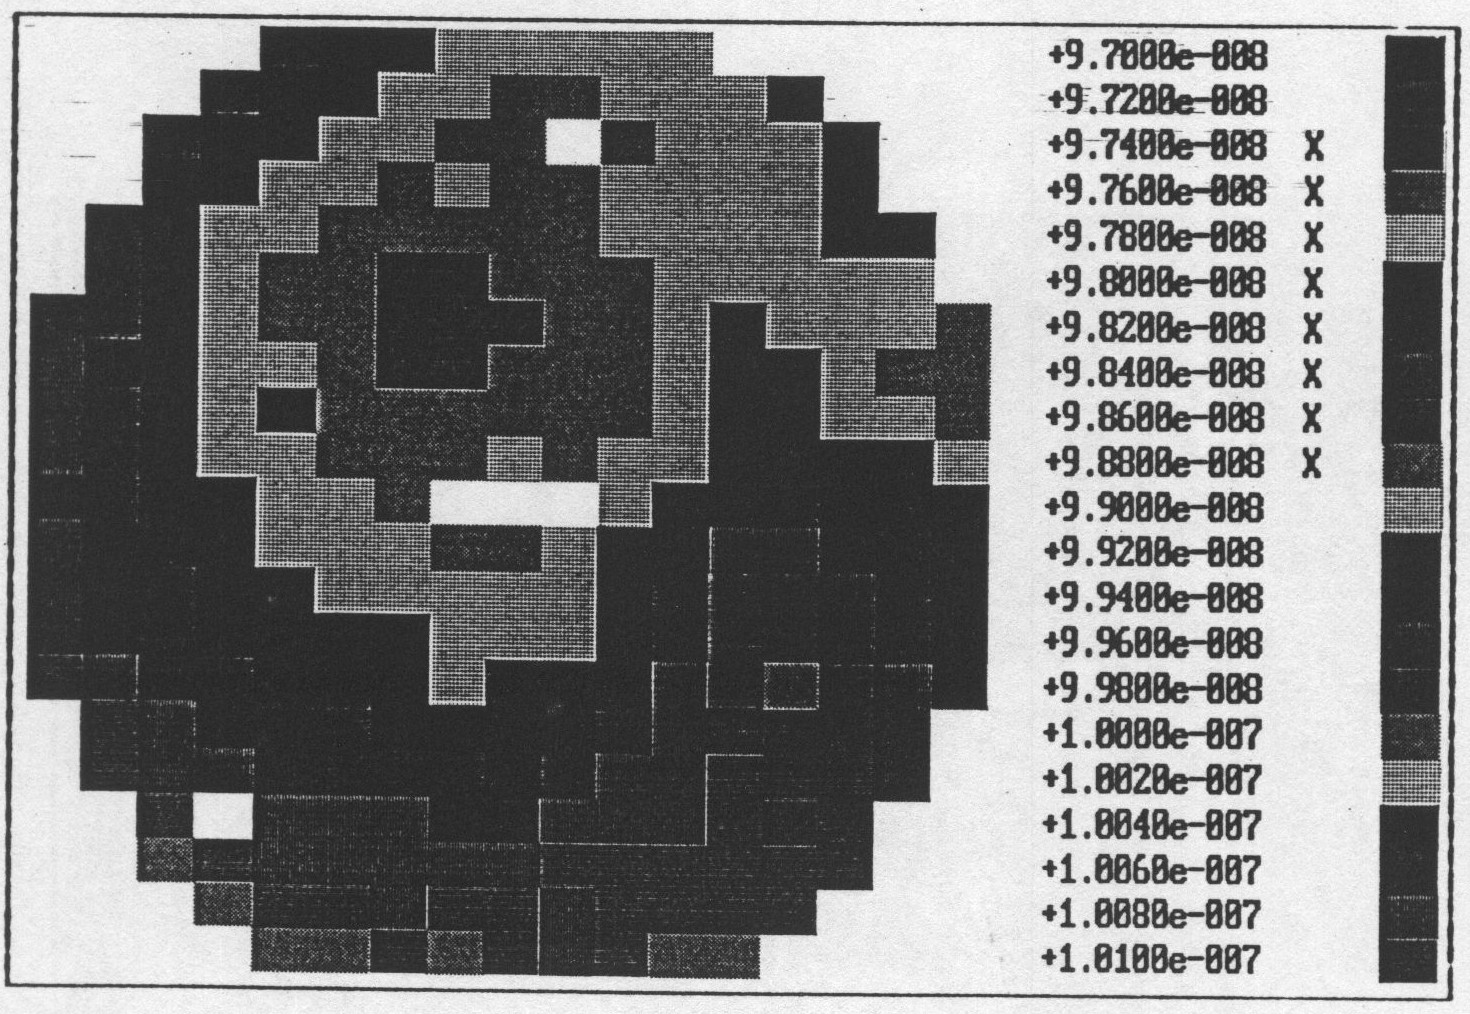
\includegraphics{Figures/fig-6-4.eps}
\captionsetup{justification=raggedright, singlelinecheck=false}
\caption[Plošné rozloženie hrúbky hradlového oxidu $h_{ox}$]{Plošné
  rozloženie hrúbky hradlového oxidu $h_{ox}$.}
\label{fig:6.4}
\end{figure}


\section{Určenie hustoty pascí rozhrania $Si-SiO_{2}$.}\label{sec:6.3}

Pre výpočet hustoty pascí rozhrania použijeme porovnanie HF a
kvázistatickej C-V závislosti, kde použijeme postup popísany v časti
\ref{sec:4.2.1}. Možno poznamenať, že pre určenie polohy Fermiho
hladiny na povrchu polovodiča použijeme hodnoty povrchového potenciálu
$\varphi_{s}(V_{g})$, získané integráciou kvázistatickej C-V
závislosti a hodnotu integračnej konštanty $\varphi_{s0}$ určíme
postupom popísaným v dodatku \ref{app:AppendixG}.

Celý postup výpočtu $D_{it}$ je realizovaný dvoma programami. Prvý program na základe zmeraných kvázistatických C-V závislostí a známych hĺbkových priebehov $N(x)$ vypočíta závislosti $\varphi_{s}(V_{g})$, ktoré uloží do dátového súboru.  Druhý program pre svoju činnosť vyžaduje dátove súbory

\begin{itemize}
\item HF C-V závislosti $C_{mos}^{HF}(V_{g})$
\item kvázistatické C-V závislosti $C_{mos}^{LF}(V_{g})$
\item závislosť povrchového potenciálu od napätia hradla $\varphi_{s}(V_{g})$.
\end{itemize}

Vypočítané hodnoty $D_{it}$ ako závislosť polohy Fermiho hladiny v
zakázanom pásme polovodiča uloží do dátoveho súboru. Na obrázku
\ref{fig:6.5} je zobrazené plošné rozloženie $D_{it}$ v strede
zakázaného pásma.

\begin{figure}[h!]\centering
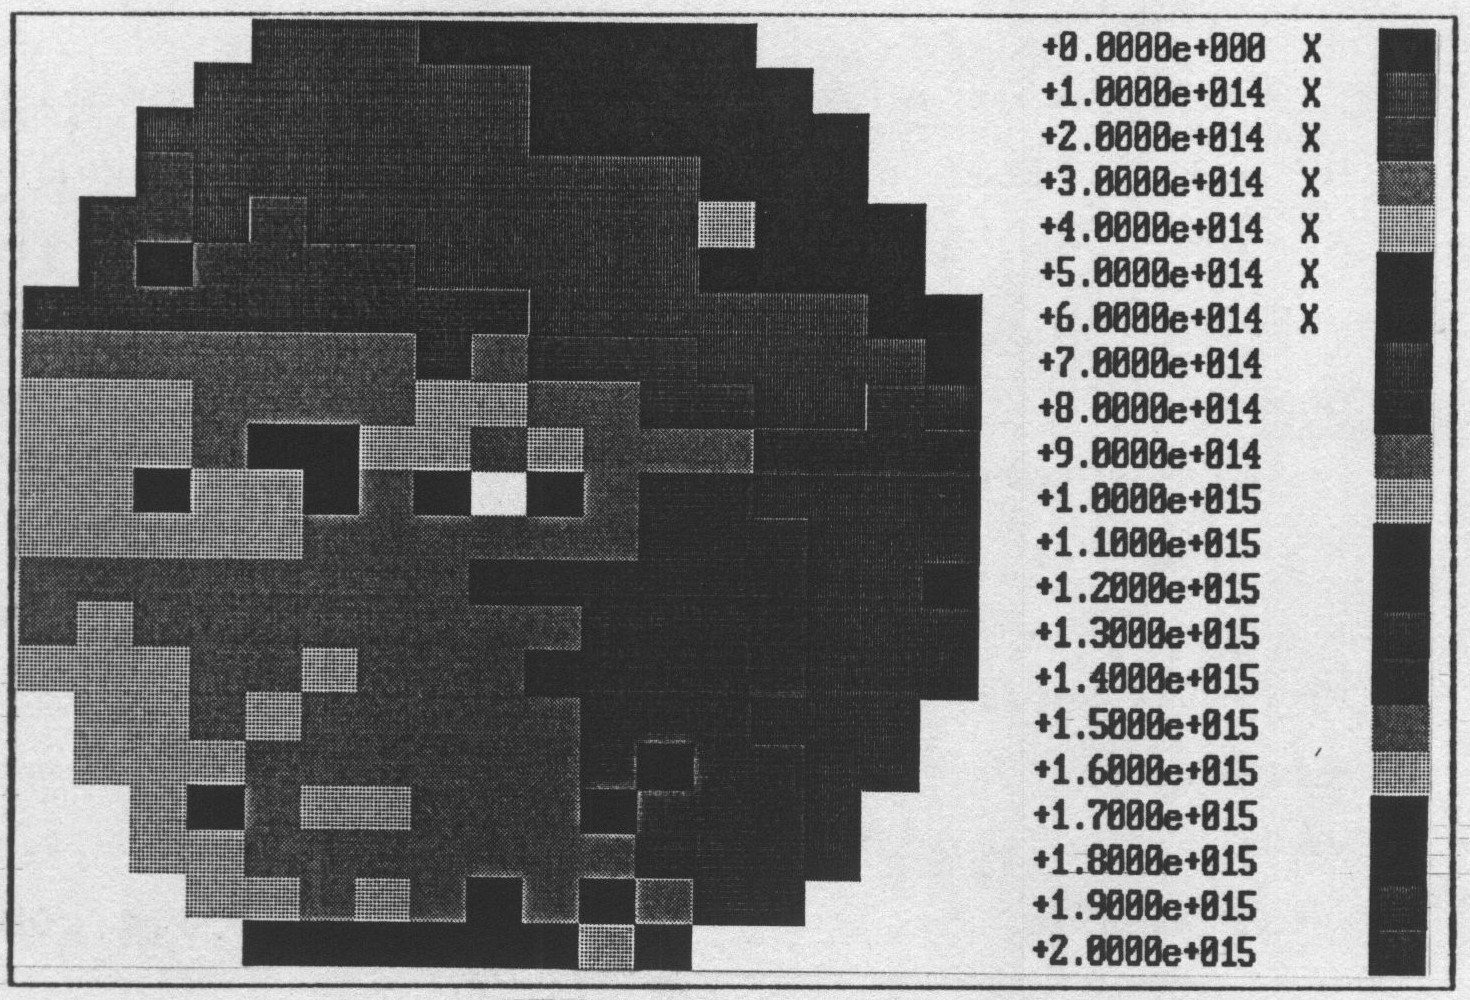
\includegraphics{Figures/fig-6-5.eps}
\captionsetup{justification=raggedright, singlelinecheck=false}
\caption[Plošné rozloženie hustoty pascí rozhrania $Si-SiO_{2}$ v
  strede zakázaného pásma]{Plošné rozloženie hustoty pascí rozhrania
  $Si-SiO_{2}$ v strede zakázaného pásma.}
\label{fig:6.5}
\end{figure}


\section{Určenie generačného času života minoritných nosičov náboja.}\label{sec:6.4}

V procese zberu dát metódou konštantnej šírky OPN bol vytvorený dátovy
súbor obsahujúci smernice závislostí $V_{g}(t)$ pre rôzne šírky OPN
testovaných štruktúr MOS kremíkovej dosky. Pre určenie generačného
času života minoritných nosičov náboja podľa vzťahu \ref{eq:3.10} je
dôležité ako vypočítame deriváciu závislosti smerníc $V_{g}(t)$ podľa
vzdialenosti hranice OPN od povrchu polovodiča. Použitie číslicových
filtrov v tomto prípade nie je vhodné, pretože máme k dispozícii málo
bodov závislosti $dV_{g}/dt = f(w)$. V tomto prípade možno pužiť
aproximáciu lokálnymi polynómami. Teoretický základ aj zdrojový text
procedúry v jazyku Algol je uvedený napríklad v \cite{6.1}. Na obrázku
\ref{fig:6.6} je zobrazené plošné rozloženie generačnej doby
minoritných nosičov náboja, ktorá predstavuje jej strednú hodnotu v
oblasti od $0.9 \mu m$ do $1.3 \mu m$.

\begin{figure}[h!]\centering
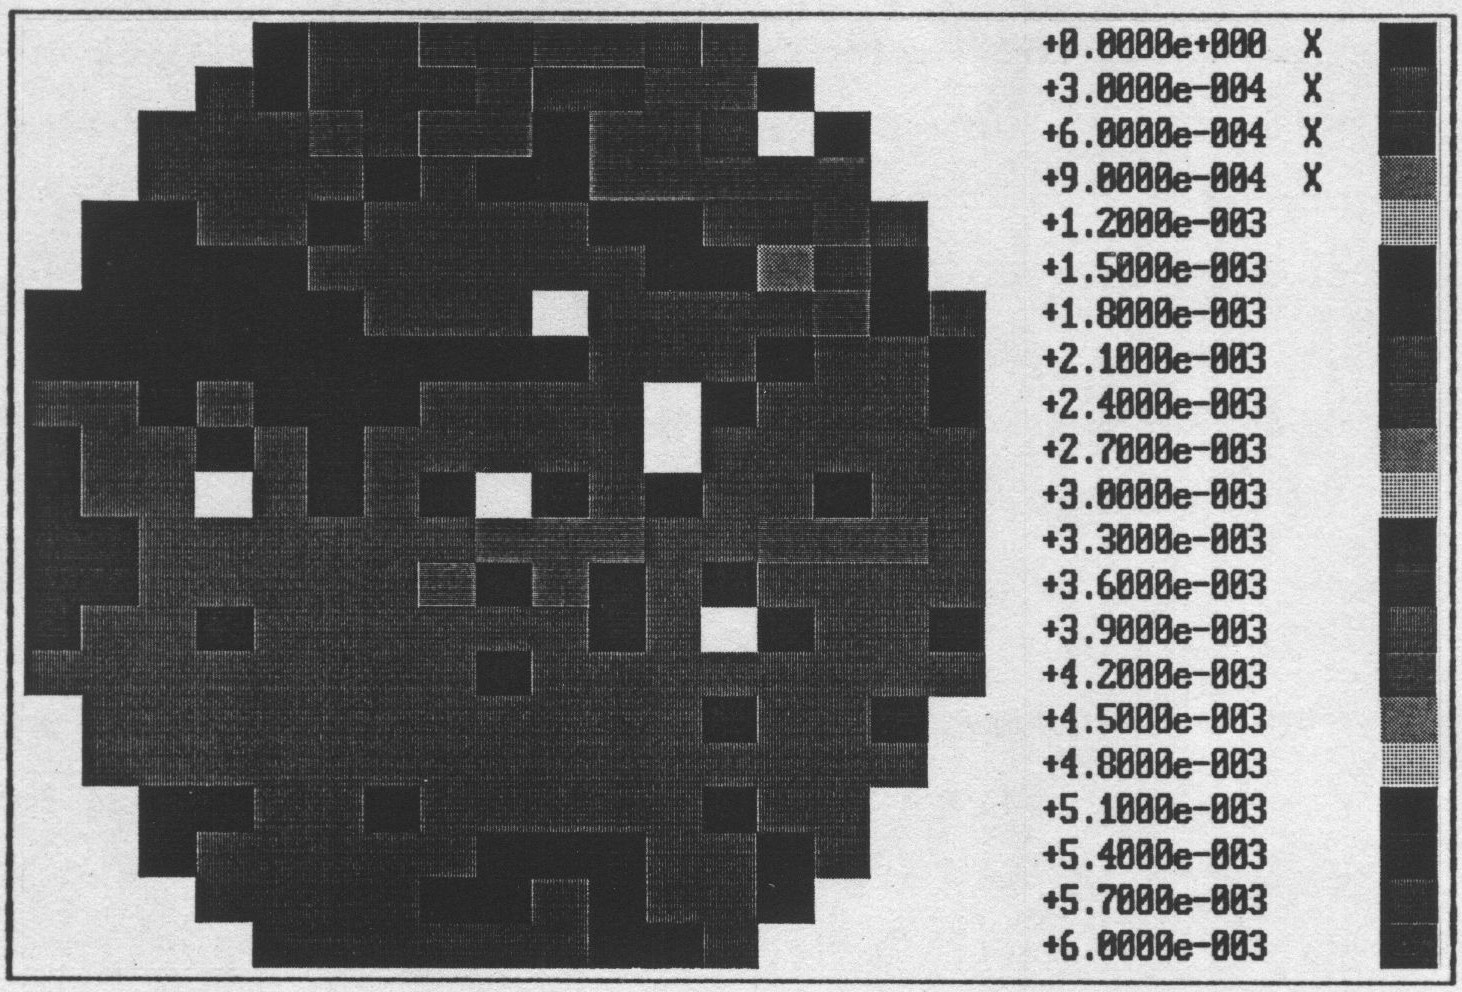
\includegraphics{Figures/fig-6-6.eps}
\captionsetup{justification=raggedright, singlelinecheck=false}
\caption[Plošné rozloženie generačného času života minoritných nosičov
  náboja]{Plošné rozloženie generačného času života minoritných
  nosičov náboja pre oblasť polovodiča od $0.9 \mu m$ do $1.3
  \mu m$.}
\label{fig:6.6}
\end{figure}

\begin{thebibliography}{}
\bibitem[6.1]{6.1}
Ludwig R.: Methoden der Fehler und Ausgleichrechnung. VEB Berlin 1969. s.103.
\end{thebibliography}
